\documentclass{exam} 
\def\workshopTitle{Workshop - Introduction} 
\input{itec625workshopHeader} 
\section*{Learning outcomes}

Following are this week's learning outcomes,
\begin{enumerate}
\item introductions
\item be ready to use the lab computers (setup accounts and iLearn)
\item your first java program
\item compiling and executing a java program
\item introduction to eclipse
\item importing a java project in eclipse 
\item adding a file to an eclipse project
\item creating an eclipse project
\item \end{enumerate}

\vspace{1em}
\begin{questions}
\question  \textbf{Access your account} \vskip 0.5cm
To log on to the lab machines, first make sure the machine is powered on. 
Enter your username (OneID) and password in the appropriate entry boxes. 
Please note that if you have already accessed the labs, your username and password are the same as in the previous semester, and if are accessing the labs for the first time, you should have the required information from enrolment/ orientation session. If you do not have this information, please ask the tutor to assist you.

Once you login to the computer, make sure you have access to ITEC625 homepage in iLearn. If not, please ask the tutor to assist you.

\newpage

\question Writing your first Java program.

In a text editor (notepad or any other editor), type the following exactly as it appears,

\begin{verbatim}
public class HelloWorld {
	public static void main(String[] args) {
		System.out.println("Hello world");
	}
}
\end{verbatim}

Save this file as \texttt{HelloWorld.java}.

Next step is to \emph{compile} and \emph{execute} the program.

The following diagram describes the process of compiling a java source code (.java) into java bytecode (.class) and then executing the bytecode on the Java Virtual Machine (JVM).
\vskip 0.5cm
\begin{center}
	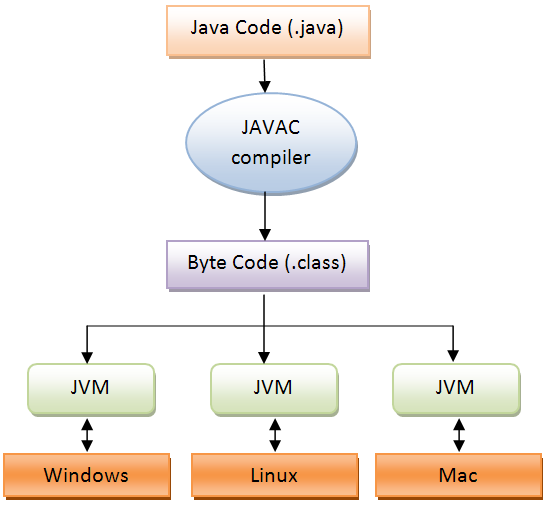
\includegraphics[scale=0.3]{javaCompileExecute}
\end{center}
\vskip 0.5cm

Open Command Prompt/ PowerShell and go to the folder in which you saved the java file. Run the following command (or \texttt{ls} on a Mac/Linux) to list the contents of the directory:

\begin{lstlisting}[numbers=none]
dir
\end{lstlisting}

You should see the file (amongst others)

\begin{lstlisting}[numbers=none]
HelloWorld.java
\end{lstlisting}

Type the following command to compile \texttt{HelloWorld.java}. 

\begin{lstlisting}[numbers=none]
javac HelloWorld.java	
\end{lstlisting}

If everything is ok, you won't see any error message and if you run the \texttt{dir} command again, you will see the additional file

\begin{lstlisting}[numbers=none]
HelloWorld.class
\end{lstlisting}

If you *do* see an error message, take a look at the error message and fix the corresponding line. Ask your peers or tutor to help you if required.

Once the errors (if any) are fixed, type the following command to run/execute \texttt{HelloWorld.class}. 

\begin{lstlisting}[numbers=none]
java HelloWorld
\end{lstlisting}

IMPORTANT: NO ".class" in the execution command.

\question \textbf{Introduction to Eclipse}

Your tutor will demonstrate the various aspects of Eclipse using a sample project.

The main aspects you should become familiar with, are,

\begin{enumerate}
	\item package explorer
		\begin{itemize}
		  	\item Project
		  	\begin{itemize}
		  		\item Package
				\begin{itemize}
		  			\item Class
				  	\begin{itemize}
		  				\item Members
					\end{itemize}
				\end{itemize}
			\end{itemize}
		\end{itemize}	
	\item console
	\item editor
	\item running a java program (a single project can have multiple runnable java programs, each called a \textit{configuration})
\end{enumerate}

\question \textbf{Importing and running Java projects in Eclipse} \vskip 0.5cm

Follow the following instructions to import Java project contained in \texttt{eclipseDemo.zip} archive file.

\begin{enumerate}
	\itemsep0.3em 
\item Download \texttt{eclipseDemo.zip}. \textbf{\color{red} DO NOT UNZIP IT} \color{black}.
\item Open \texttt{Eclipse} IDE. A shortcut for it should be located on your desktop.
\item If prompted, set your \texttt{workspace} (a location where all your projects will be saved). We suggest you use a dedicated folder in your network drive as the workspace.
\item Click on \color{blue} File --> Import --> General --> Existing Projects into workspace \color{red} (and NOT ``Archive file") \color{black}.
\item On the next window, choose ``Select archive file'' option and browse for the archive file \texttt{eclipseDemo.zip} and choose \texttt{Open}.
\item It should show a project \texttt{basicJavaProject}. Click on \texttt{Finish}.
\item You should see a project in Eclipse in the left panel (\texttt{Package Explorer}).
\item Double click on the \texttt{basicJavaProject} to reveal \texttt{src}. \texttt{"src"} is short for \texttt{"source"} (that is, source code).
\item Double click on the \texttt{src} to reveal package \texttt{"(default package)"}.
\item Double click on the \texttt{(default package)} to reveal three source files. Run them in the order below. Your tutor will help you on how to run these files.

	\begin{enumerate}
		\item Program1
		\item Variables
		\item Expressions
	\end{enumerate} 
\end{enumerate}

\question Adding a new source file to an existing project.

In the project \texttt{basicJavaProject}, add a new source file by right-clicking on \texttt{(default project)} (in the left panel known as package explorer), choosing \texttt{New} and then \texttt{Class}. Name it \texttt{MyFirstClass} and \textbf{make sure to check} the \texttt{public static void main(String[] args)} inclusion option. Add a few lines of code from what you've learnt in the last three programs. Show this to your tutor.

\question \textbf{Creating a new Eclipse Java Project}

You can create a new java project in Eclipse by following the steps listed below,

	\begin{enumerate}
	\item Click on \texttt{File}
	\item Choose \texttt{New}
	\item Choose \texttt{Java project} (not \texttt{Project})
	\item Name the project \texttt{myFirstJavaProject} (project names begin with lowercases and are camelCased)	
	\end{enumerate}

Then you can add a new file to the project as explained in the previous question.
\end{questions}

\newpage

\section*{Advanced questions}

Some students might have done a fair bit of programming beforehand. These students should complete the following tasks.

\begin{questions}
\question acquaint themselves with the debugger feature of eclipse. create a java project and add a file \texttt{Service} containing the \texttt{main} method in it. Add a second method with the template:

\begin{lstlisting}
/**
 @param: n (assume n >= 0)
 @return: sum of the first n powers of 2.
 that is, 2^0 + 2^1 + 2^2 + ... 2^n.
 Note that the value of this series is 2^(n+1) - 1 
 but you shouldn't use this. 
 Instead, compute the value iteratively using a loop
*/
public static int sumPowersOfTwo(int n) {
	return 0; //to be completed
}
\end{lstlisting}

Next, call the method in the \texttt{main} method by passing it a value 10. The value returned should be printed on the console and should be 2047. Try it for 15. It should be 65535. Try it for 25. Till when is the value valid? Why do you think it becomes invalid after a certain value of \texttt{n}?
\end{questions}
\end{document}
